\chapter{The Maturation of Arcus}
\label{chapter:arcus}

\begin{quote}
``If you want to have good ideas you must have many ideas. Most of them will be wrong, and what you have to learn is which ones to throw away.'' \\
--- \textit{Linus Pauling}
\end{quote}

\section{Introduction}

This chapter describes the culmination of all work that has been performed for this dissertation. Following the systematic testing of \prearcus\ a number of short-comings were identified and attempts have subsequently been made to rectify them. The first few sections in this chapter begin by describing, in general terms, the algorithmic enhancements that have been implemented. The precise implemented logic used to combine these features into version 1.0 of \arcus,  is concisely defined  in section \ref{section:arcus:exactImplementation}. Finally, the predictive-performance of \arcus\ is presented and final conclusions drawn.


\section{Sampling Conformational Space}

\prearcus\ was initially used to explore the idea of the exhaustive enumeration of a coarse-grained \angleset. This exhaustive enumeration guaranteed that all of the coarse conformational space was assessed. It was originally intended that a search method of this coarse space would be developed and subsequently parametised. The method would likely have been an evolutionary MC algorithm such as that used in the previous \raft\ study\cite{COMPCHEM:Gib2001}. Following testing, however, the development of such a conformer-based sampling method was abandoned. Using the evidence presented in chapters \ref{chapter:casp} and \ref{chapter:methods} and in agreement with other published findings\cite{METHOD:Plop,METHOD:RapperB}, it was concluded that the use of a coarse-grained \angleset\ is insufficient \emph{in the context of} surface-loop modelling. This ultimately stems from fact that a coarse representation is often unable to allow valid conformations, when the \mainchain\ path is required to \emph{simultaneously} connect two well-defined points and satisfy both geometry and steric interactions.
In light of this, the following section details how \arcus\ deviates from the pure use of an \angleset.

\subsection{Main-chain Torsion Library Granularity}

In chapter \ref{chapter:methods}
a general trend was identified, in which methods based upon fine-grained \mainchain\ torsion libraries seemed to exhibit significantly higher predictive performance than those based upon coarse-grained libraries. It now seems clear that this is primarily due to the fact that, in torsional space, many native-like conformations  are screened  early in the modelling process by steric filters. This is primarily due to small \emph{concerted} deviations from native \mainchain\ torsions, that ultimately yield large deviations in Cartesian conformation -- termed the ``lever effect''. By allowing deviation from the exact parametised values, it was hoped that more native-like conformations could be kept. The caveat to this, of course, is that a greater variety of non-native conformations are also generated. In light of this, enhanced heuristic filtering and sampling were also required and are described in section \ref{section:arcus:filterdev}.

This lever-effect can also partially explain the recurring tendency of \prearcus\ to produce over-extended loop candidates that reach far from the protein body. As extended structures inevitably pass steric filters and there are no additional filters to remove non-compact states, there will be proportionately more ``valid'' extended conformations than those which are compact. Again, additional heuristic filters are evidently required, as \ambergbsa\ alone seem unable to discriminate against these over-extended states.
Removal of such non-native states is also highly beneficial for the search efficiency, as less time is spent exploring invalid states in the later stages.
\subsection{Sampling}

An \emph{exhaustive enumeration} of a fine-grained \angleset\ is computationally unfeasible. However, the comparative cost of \emph{sampling} larger \anglesets\ can be less than that of an exhaustive enumeration of a coarse-grained \angleset. By using quick and computationally efficient filters, many clashing or unlikely conformers may be discarded very early in the modelling process. This makes the evaluation of such conformations extremely cheap.
These filters can be \emph{more stringent} than those used in \prearcus\ as there is a reduced likelihood of no native-like conformation being generated.

In the knowledge that fine-grained torsional sampling is desirable, a number of important procedural enhancements have been made. Firstly, the propensity-weighting information derived for the \angleset\ is now utilised to bias sampling. Secondly, the larger optimised 8-10-5 \angleset\ has been employed, better representing the populated regions of conformational space and requiring a smaller search radius around parametised angle-pairs. Thirdly, the tweak-store has been replaced by ``noise'', introduced into the next() function of the \textsl{ConformerBuilder} -- the noise  is simply a normally-distributed random value added to each parametised angle-pair prior to application. The $\sigma$ of the random perturbation was set at 15\degree\ to effectively give a maximum deviation of approximately 50\degree, due to  the recommendation stated in section \ref{section:reduced_rep:optimised_angleset}.



\subsection{Dual-branch Conformers}
\label{section:arcus:dualbranch}


To alleviate the lever-effect further, a change of tactic in the \textsl{ConformerBuilder} was implemented. As employed by other methods\cite{METHOD:Plop,METHOD:CLOOP}, the conformer was split at the central amino acid, as opposed to the C-terminus. When the conformer contained an odd number of residues, the extra residue was assigned to the N-terminal branch. The break itself was re-positioned across the peptide group between the two central amino acids. All other components of the algorithm were then adapted to accommodate this change in break definition. As the conformers are now half the length, the lever-effect is less pronounced. A single conformer-descriptor can still be used to represent a single loop, but now rather than representing the path leading from the N-terminus, it represents two half-paths extending from either terminus.
A second advantage of this change is increased efficiency, as fewer atoms are required to be transformed per rotation.

\subsection{Implementation}

The changes outlined thus far are actually less of a deviation from the original implementation of \prearcus\ than it might seem. The original \textsl{ConformerBuilder} computer code was designed with versatility in mind, simply with the primary ability to rapidly apply torsional changes to a section of protein \mainchain. This segment was defined, with a single break at one end, to be re-joined later. By deriving from the \mbox{\textsl{ConformerBuilderBase}} class, it is possible to completely redefine the controller logic with minimal additional coding effort. The same fundamental \anglesets\ can also still be used as the basis for the search, but this time allowing deviations around these angles during the \emph{stage 1} search as opposed to stage 2 onwards.
















\section{Filter Enhancements}
\label{section:arcus:filterdev}

Compared to \prearcus, the filters used in \arcus\ are far more stringent and comprehensive. The specific new filter types are discussed in detail below.


\subsection{Principles for Filtering}

As described in chapter \ref{chapter:prearcus}, in \prearcus,\ a rapid exhaustive enumeration of the coarse-grained \angleset\ was performed for each candidate loop. Those passing the series of filter-based cut-offs were kept for entry into stage 2. As described in chapter  \ref{chapter:prearcus}, the filters had to be of the correct balance to keep enough conformations to cover at least one native-like state whilst at the same time not introducing too many additional conformations to stage 2 of the re-modelling process; being more  computationally expensive.  

Following testing, it was found that simple fixed cutoffs are not ideal in this endeavour, with some test loops yielding tens of valid conformers and others producing tens of thousands.
In hindsight this is expected, as in nature some surface loop structures are known to be more naturally flexible than others. Conformational flexibility is highly dependent both on the loop sequence and on the nature of the underlying protein body.


An adaptive filtering system was thus required. The developed procedure executes stage 1 until a buffer has been filled with a sufficiently diverse series of candidate conformations before stage 2 is invoked. As stage 1 is comparatively cheap, it is desirable to spend proportionately more effort ensuring a higher quality of candidate structure, rather than relying too heavily on the torsional minimisation of stage 2 to resolve clashing conformations.

In addition to this, it is thought that the physical determinants of the energy landscape are predominantly steric in nature. Electrostatic interactions are thought to fine-tune the relative stability of sterically viable competing minima. Thus, a steric-filter-based \mbox{stage 1} is desirable, prior to assessment with a \forcefield\ capable of describing electrostatic interactions.

\subsection{Additional Stage 1 Filters}

The filters used in stage 1 of \prearcus\ remained predominantly unchanged in \arcus\ aside from some computational efficiency improvements  and the use of smaller cut-offs.
The main change is the addition of new filters for the search process, which are outlined in the following sections.




\subsection{The Branch-Distance Filter}
\label{section:arcus:branchDistFilter}

The branch-distance filter functions on the principle that if  a given branch of the conformer strays too far from the opposite anchor, there is no conformation of the other branch that can ultimately result in a joined pair. Branches which do stray too far can then, by definition, be removed from the search process.
In order to filter based upon this criterion, \thothloopdb\ was used as the data source for the required parameters. 

The first stage was to define a set of distances that could be rapidly measured during conformer selection, as a way to filter those with inappropriate orientation. Square-distance comparisons were used, as the basis for the filter, due to their computational efficiency. Figure \ref{fig:arcus:segfan} shows how vectors were defined based upon the position of the two proximal anchor residues with respect to the loop. Two anchor-orientation vectors were defined as  the \ca--\,\ca\ vector and the C--N vector between the two anchor residues. The difference between these two distances, $\Delta$-Anchor, describes the relative direction of the two anchor residues -- the observed extremes are shown in  figure \ref{fig:arcus:segmaxmin}. These two distances can thus be used to describe the ``anchor-environment'' for a given loop. Following this, the distance deviation from each \ca-atom within the loop to the \emph{opposite} anchor atom is calculated. Here, the ``opposite atom'' was defined as N and C-atoms for the N and C-terminal branches respectively. When there is an odd number of residues, the final single-residue is deemed part of the N-terminal branch. Each of these distances were pre-calculated for all known loop structures within \thothloopdb. 

When the filter is initialised, it measures the two orientation vectors for the current anchor configuration. It then searches the database for all examples of the same loop length with an anchor-separation and $\Delta$-Anchor within $\pm2.0$\AA\ and $\pm$0.2\AA\ respectively. At least 15 database examples must be found, otherwise the cut-offs are incremented by 0.2\AA\ and 0.02\AA\ respectively until enough examples are found, or until 10 attempts have been made. These anchor cutoffs were chosen by eye from graphs similar to those in figure \ref{fig:arcus:segsymmetry}.
If not enough examples are found, the program exits with an error condition.
Once all similar examples are found within the database, the extreme observed distance separations are obtained for each \ca-atom position within the candidate loop, relative to the opposite anchor atom.  Any generated conformations which have one or more measured distances outside these extremes are eliminated.

\begin{figure}[hbtp]
\begin{center}
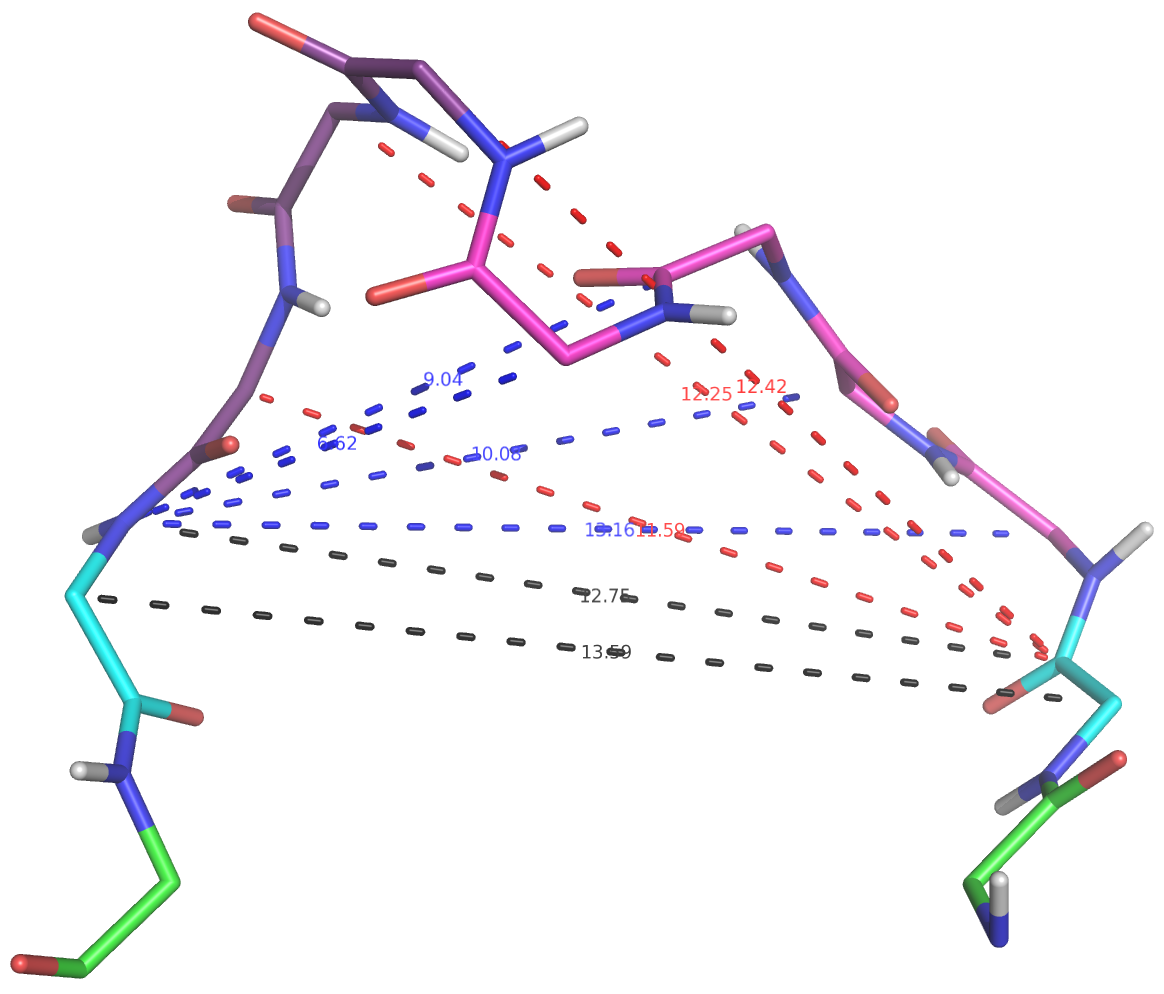
\includegraphics[width=0.7\textwidth]{09-Arcus/segdist/seg_fan.png}
\end{center}
\caption[A typical joined \mer{7} loop segment]{A typical joined \mer{7} loop segment is shown, with the N and C-terminal halves in dark-magenta and magenta respectively. 
The two closest anchor-residues are shown in cyan, with other immediate residues in green. The two primary vectors which define the
anchor separation and orientation, the \ca--\,\ca\ vector and the C--N vector, are shown as black dashed lines. 
Finally, the radial distances from the N-terminal anchor atom to each \mbox{\ca-atom} in the opposite half of the loop are shown as blue dashed lines. The equivalent lines for the C-terminal branch are shown in red.}
\label{fig:arcus:segfan}
\end{figure}

\begin{figure}[hbtp]
\begin{center}
\subfigure[Minimum $\Delta$-Anchor found: Sequence GYWNLDMMTF, taken from 2A15A. A very negative separation value of $-1.848$\AA, representing anchor vectors which point away from other.]{
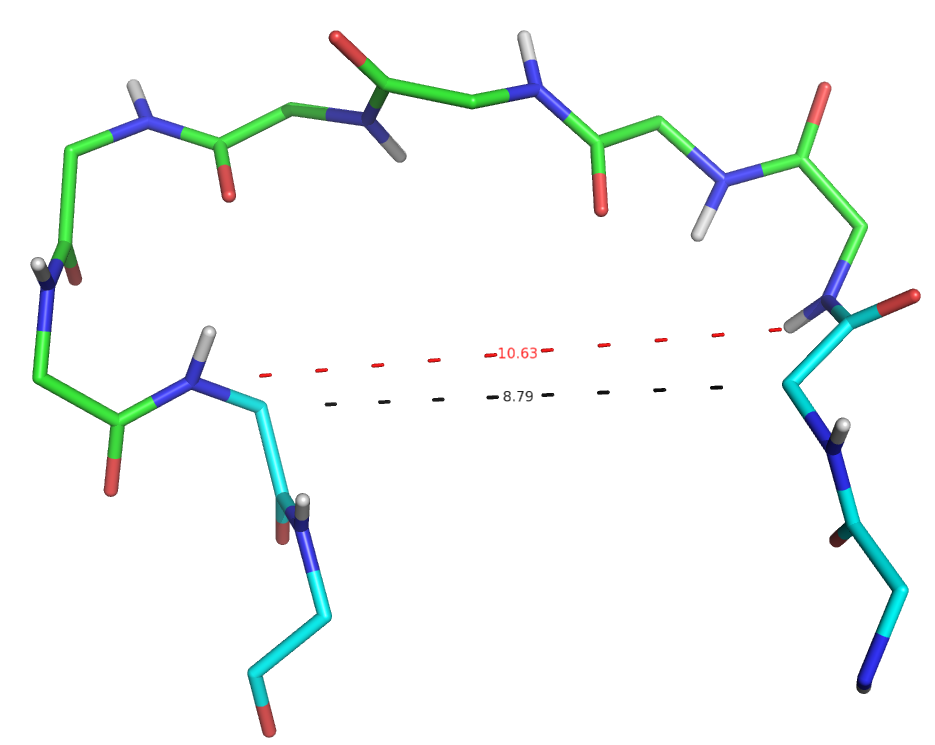
\includegraphics[width=0.35\textwidth]{09-Arcus/segdist/min.png}
}
\quad
\subfigure[Maximum $\Delta$-Anchor found: Sequence RLETGRTHQI, taken from 1V9FA. A very positive separation value of 2.890\AA, representing anchor vectors which point towards each other.]{
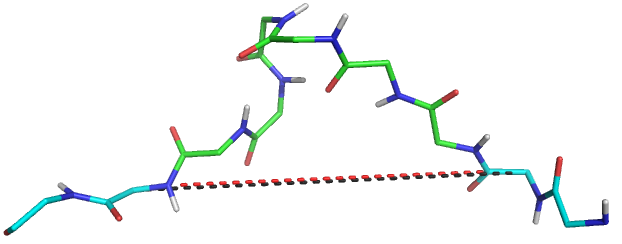
\includegraphics[width=0.545\textwidth]{09-Arcus/segdist/max.png}
}
\end{center}
\caption[The effect of $\Delta$-Anchor on loop-orientation]{The effect of $\Delta$-Anchor on loop-orientation. Each image illustrates a \mer{6} loop, shown in green, with four anchor residues shown in blue.}
\label{fig:arcus:segmaxmin}
\end{figure}

One final decision must be made. One must decide whether the N and-C terminal branches are structurally equivalent in terms of the derived distance extremes. Figure \ref{fig:arcus:segsymmetry} shows that separate treatment is \emph{not} required, as the distributions are essentially identical. Thus, the 1 and $n$, the 2 and $n-1$ and  ... the j and $n-j+1$ positions are considered structurally equivalent for this purpose; where $n$ is the number of residues in the loop. The positions are not actually equivalent, but here gross averaging of the data is performed and so such considerations are void. This is also advantageous, because it doubles the data density within the pre-calculated database for each residue position.

The final filter definition for the loop being built is thus:

\begin{figure}[hbtp]
\begin{center}
\subfigure[Data from residue position-1 only]{
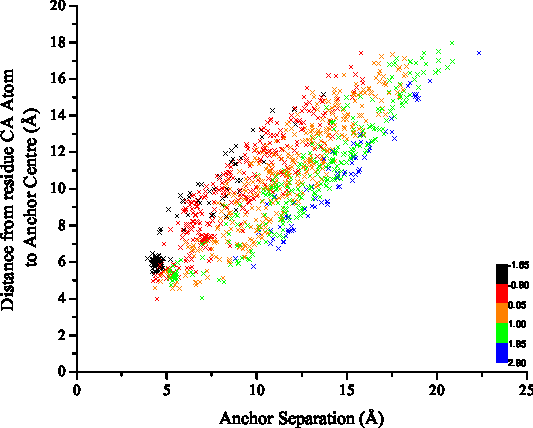
\includegraphics[width=0.47\textwidth]{09-Arcus/segdist_graph/pos1_just1.pdf}
}
\subfigure[Data from residue position ``Nearest Anchor +1'']{
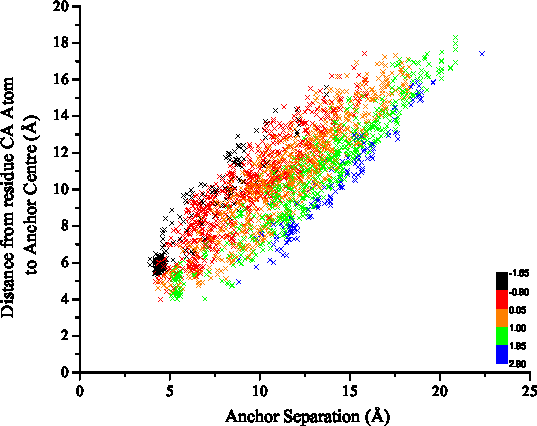
\includegraphics[width=0.478\textwidth]{09-Arcus/segdist_graph/pos1_both.pdf}
}
\subfigure[Data from residue position-2 only]{
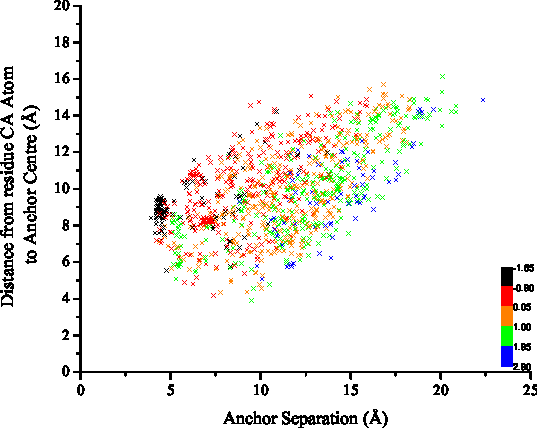
\includegraphics[width=0.47\textwidth]{09-Arcus/segdist_graph/pos2_just2.pdf}
}
\subfigure[Data from residue position ``Nearest Anchor +2'']{
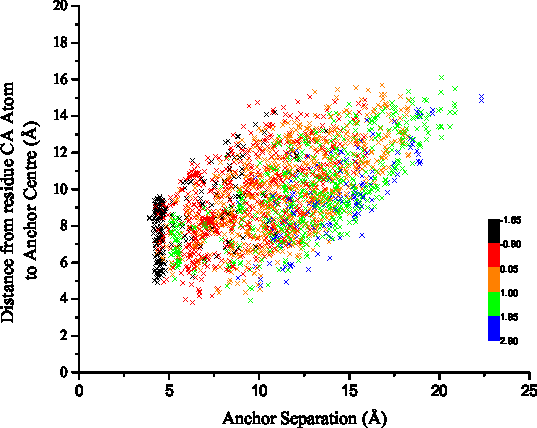
\includegraphics[width=0.478\textwidth]{09-Arcus/segdist_graph/pos2_both.pdf}
}
\subfigure[Data from residue position-3 only]{
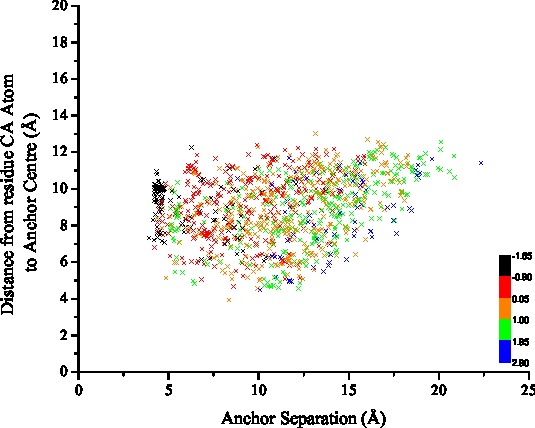
\includegraphics[width=0.47\textwidth]{09-Arcus/segdist_graph/pos3_just3.pdf}
}
\subfigure[Data from residue position ``Nearest Anchor +3'']{
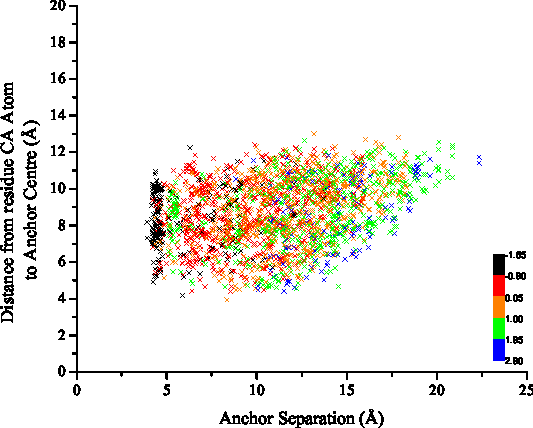
\includegraphics[width=0.474\textwidth]{09-Arcus/segdist_graph/pos3_both.pdf}
}
\end{center}
\caption[Data for \mer{6} loops from \thothloopdb]{Branch-distance data for \mer{6} loops from \thothloopdb. The colouration signifies the value of $\Delta$-Anchor, as defined by the graph key. A negative $\Delta$-Anchor signifies that the anchors point away from each other, a positive value, the opposite. Clear banding can be seen in the distributions, showing that the use of $\Delta$-Anchor and anchor-separation can potentially yield discriminatory power in conformer selection. The similarity of the left-hand graphs to those directly to the right, illustrates that the conformational freedom of the N and C-terminal halves is approximately equivalent, for any corresponding residue positions.}
\label{fig:arcus:segsymmetry}
\end{figure}
\begin{enumerate} \isep
\item Measure the distance between the \ca-atoms for the two anchor residues.
\item Measure the distance between the C and N \mainchain\ atoms for the N and C-terminal anchors respectively. Subtracting the second distance from the first defines $\Delta$-Anchor.
\item Look-up distance data from the database, corresponding to the same loop length and anchor orientation. Within reasonable certainty, this defines the maximum and minimum distances for each loop \ca-atom to the opposite anchor atom encountered within the actual PDB. 
\item For each maximum and minimum, add and subtract 5\% respectively, to allow a degree of lenience for model structures. Next, square the two values, as distances are compared as their squares
for computational efficiency.\item During conformer selection, for each residue position, compare the current square-distance to the maximum and minimum allowed distances for that position. Discard all conformations for which any single measured distance is outside its allowed range.
\end{enumerate}

\subsection{The Over-Extension Filter}
\label{section:arcus:overExtFilter}

To combat the over-extension problem, a value for the maximum-reach away from the protein body for surface loops,  was obtained from the literature\cite{METHOD:Plop}. This was then used as a conformational cut-off, forcing the population of valid stage 1 conformers to be less solvent-exposed.
From this, a user-adjustable cut-off with a default value of 6.32\AA, was assigned as the minimum distance from a loop \mainchain\ atom to any heavy-atom in the protein body. The cutoff was applied to all residues greater than one position away from the anchors, as the closest residues implicitly pass the filter. Any conformation which had a minimum distance in excess of this cut-off, for any single \mainchain\ atom, was discarded outright. This default value covers $\sim$99.0\% of native loop structures. Less stringent values would provide yet greater coverage, but also allow a greater relative proportion of non-native structures. Therefore, a less stringent cut-off effectively decreases the signal-to-noise ratio for the majority of loop predictions and thus would result in poorer predictions in some cases.

\subsection{Steric Clash-grid Filter}
\label{section:arcus:clashGridFilter}

\prearcus\ used a simple mechanism for clash detection. For performance reasons, the original clash-filter used a ``surface-box'' containing \emph{only} \ca\ atoms for steric tests, originally illustrated in figure \ref{fig:reduced_rep:surface}.
Each \ca-atom in the loop was compared to each \mbox{\ca-atom} in the local protein body to see if the hard spheres overlapped by more than a given proportion. For this reason, significant clashes could occasionally remain unfiltered, even though the loop conformation exhibited only minimal \ca-atom clashes, caused by an undetected \mainchain\ or \sidechain\ clash. In the new version,
all protein core heavy-atoms are used in clash-detection.

This became possible owing to the implementation of a cell-list.
This superior method involves the creation of a fine grid around the moving loop atoms. For each individual point on the grid, the atoms within a given cut-off, defined as 3.5\AA\ here, are added to its list. All that is then required during loop simulation is the dynamic selection of the closest grid point for each loop atom. The specific list can then be retrieved and only those atoms assessed for clashes. As one lookup is required per loop atom and the index-lists are precalculated, this improved algorithm scales linearly with increasing protein size.

Importantly, the rotamer packing routine is now called following the building of the \mainchain\ conformation.
The grid-based clash detection routine is then recalled for all heavy-atoms within the loop. Unlike \prearcus, this ensures that there is sufficient volume for each \sidechain\ to occupy, prior to the invocation of the stage 2 torsional minimisation.
\subsection{Filter Summary}

Conformers generated under the new sampling method can be more proficient in the satisfaction of spatial restraints and steric interactions. The stringency of the \mbox{stage 1} filters has, therefore, been increased. As a larger proportion of generated conformations are filtered, the conformations which still pass are of higher quality. As stages-2 and 3 are more computationally costly than stage 1, the generation of larger numbers of conformers under harsher filters makes sense from the point of view of \emph{overall} efficiency of \arcus. 

This fundamental change also had the positive side-effect that the stage 2 torsional minimisation is relied upon to a lesser extent to resolve the balance between join-distance and steric interactions. Section \ref{section:casp:torsionalMinimisation} concluded that an element of the over-extension problem was that poor conformations were pushed away from the protein body and into solvent by the torsional minimisation protocol. This difficulty is now, therefore, resolved.


\section{Improved Rotamer Packing}
\label{section:arcus:impRotPack}

\prearcus\ employed randomised, sterically-guided rotamer application and torsional perturbation as the basis of its \sidechain\ packing procedure. Whilst it was evidently capable of finding low-energy conformations, the nature of the packing process was largely inefficient, requiring multiple torsional minimisations in order to find well-packed states. Core \sidechain\ packing was, therefore, sometimes sub-optimal with respect to the native state. A way of very rapidly packing rotamers to a defined state per \mainchain\ conformation change was required, rather than relying upon the costly MC-based procedure. 

A rotamer-packing mechanism has been implemented for this work and is described in the remainder of this section. The MC procedure is now therefore, charged solely with \mainchain\ sampling. A perturbation can be enabled which triggers \textsc{Scwrl} \sidechain\ packing. This ensures that the simulation retains high-quality packing of high probability \sidechain\ conformations.

\subsection{Implementation Options}

\textsc{Scwrl}\cite{METHOD:SCWRL_1} is one of the most rapid and effective rotamer assignment algorithms currently available and currently stands at version 3.0\cite{METHOD:SCWRL_2}.
The authors report that the algorithm is capable of assigning complete \sidechain\ predictions for 180 proteins, involving 34,342 individual \sidechains, in under 7 minutes on a dual AMD MP1800+. The current version evaluates potential rotamers using steric interactions and probability data alone. Nonetheless, when using the standard implementation that has been reproduced for this work, the predictive capability of the algorithm is reported to be 82.6\% and 73.7\% for $\chi$-1 and $\chi$-2 respectively.

The recent algorithm  \textsc{Andante}\cite{METHOD:ANDANTE} is a highly effective alternative, but is directly influenced by the \sidechain\ conformation information in homologous proteins. \textsc{Andante} is therefore both less applicable to surface loops and uses information which is  not available within a pure \abinitio\ builder, such as \arcus. \textsc{Scwrl} is therefore the logical choice of rotamer packing algorithm for use in conjunction with the other elements of \arcus.

Whilst the \textsc{Scwrl} software itself is freely available to academics, the source code is not. As such, use of the algorithm during loop modelling required re-implementation from the original papers. The rotamer library and application system in \pd\ was substantially re-written to allow implementation of the \textsc{Scwrl} algorithm and the incorporation of support for backbone-dependent rotamer libraries -- a feature that was previously missing. In the new implementation of the algorithm in \pd, the rotamer library is de-convoluted from the process of rotamer selection, thus any implemented rotamer library may be used with any implemented search process. The newer, more sophisticated code can apply individual rotamers an order-of-magnitude more quickly than the previous version; even before any algorithmic enhancements for rotamer selection are taken into account.



\subsection{Graph-Theory Terminology}

\textsc{Scwrl} makes use of graph-theory algorithms in order to rapidly find the \emph{global} minimum with respect to its energy function. As such algorithms are discussed below, basic graph-theory terminology is defined here. Graph theory is simply the treatment of a system as a graph ($\mathcal{G}$), composed of a series of vertices ($\mathcal{V}$)
and a series of edges ($\mathcal{E}$) that connect them. The \emph{adjacency list}
of a given vertex is a list of vertices with which it shares an edge.
The graph is said to be \emph{undirected} if there is no directionality for any of the edges.
For an interacting pair of vertices, where $v$ and $w$ are the tail and head respectively, $v \rightarrow w$ defines an edge connecting the two vertices, whereas $v \overset{*}{\rightarrow} w$ defines that there is a connected path of one or more edges between them.
A \emph{simple cycle} is defined as a closed path, with no repeated vertices apart from the starting and ending vertex. Any connected graph with no cycles is a \emph{tree}.
From any defined staring node with one associated edge, termed the root, one can descend 
to any given leaf-node.

Two vertices are in the same connected-component if, and only if, there exists a path between them. In graph theory, a \emph{biconnected component}  is defined as a maximal set of edges of a connected graph such that any two members lie on a common simple cycle.
In other words, at least two vertices must be removed from a biconnected component in order to separate
it into two connected components.
Articulation points are defined as those vertices which form a bridge between two biconnected components. The order of an articulation point is defined as the number of biconnected components to which it is bound, minus one. 



\subsection{Choice Rotamer Library}

There is a large choice of possible rotamer libraries available for use in modelling, provided by a number of different academic groups.
A leader in the field is Dunbrack who's group supplies both backbone conformation-dependent and independent rotamer libraries\cite{NATIVE:Dunbrack2002}. An alternative is the Penultimate Rotamer Library by the Richardson group\cite{COMPCHEM:RICHARDSON}.
Both of these libraries  define rotamers by a series of $\chi$-torsions with associated backbone propensity information. Finally, Shetty et al provide a library based upon clustered Cartesian conformations with associated grid-based backbone propensity maps\cite{NATIVE:Shetty2003}. This paper then goes on to discuss the advantages of fine-grained rotamer libraries. For the remainder of this work the Shetty library is used, although the Dunbrack libraries were also implemented for trial in future works. 

The high-quality Shetty library was chosen due to two primary advantages. The first is that three progressively more fine-grained libraries are supplied, which are derived from three increasingly tight Cartesian clustering cutoffs. These libraries can each be utilised, as appropriate, at different times during the modelling process to give an increasingly more detailed ensemble of viable \sidechain\ conformations. The second consideration was that, following optimisation and benchmarking, the \pd\ rotamer-application code, which is capable of applying rotamers in either torsional or Cartesian space was found to be faster when applying Cartesian coordinates. Thus, there is no advantage in the use of a torsional library, which by definition averages out any bond and angle deviations.  In fact, these deviations most likely play an important role in some specialised \sidechain\ conformations. Example ensembles from the library are shown in figure \ref{fig:arcus:shetty}.

\begin{figure}[htpb]
\begin{center}
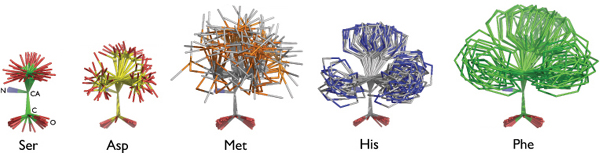
\includegraphics[width=0.9\textwidth]{./09-Arcus/shetty/shetty.png}
\caption[Structural examples from the Shetty rotamer library.]{Structural examples from the Shetty et al rotamer library. Image from\cite{NATIVE:Shetty2003}.}
\label{fig:arcus:shetty}
\end{center}
\end{figure}

\subsection{The Fundamentals of the SCWRL Algorithm}

The \textsc{Scwrl} algorithm is capable of rapidly selecting between a large number of possible rotameric states based, by default, upon steric and probability criteria.
As described, the Shetty backbone-sensitive rotamer library was selected for use in this work in combination with the \textsc{Scwrl} packing algorithm;  as opposed to the backbone-dependent Dunbrack library employed by the official version.
The algorithm itself involves a series of steps which systematically eliminate large numbers of rotamers from the search process, without the need for any heuristic filters to make the algorithm computationally tractable. Such filters could, of course, deny the search process from finding the global minimum of its own energy function. Each stage of the process is described briefly below. Some of the individual components are then described in greater detail in the following sub-sections.

The algorithm begins with a cull of any rotamers which reside within the least likely 10\% of possible states. It was found in the original work that the use of these states yields no advantage in terms of prediction accuracy, but had a significant detrimental effect on the performance of the algorithm, as many pairwise comparisons are made during the search process.
In the \pd\ implementation, custom rotamer filters can be applied at this point by the user. This allows the user to ensure that specific single rotamers or arbitrary types of rotamers are removed from the remainder of the search process, if desired.
Steric interactions between all active rotamers are then pre-computed
as they are often required by the following calculations.

Next, rotamer states are filtered by a process of dead-end elimination (DEE) using the ``Goldstein criterion''. This is the most simple of the DEE\ criteria, but proves to be highly effective. A proposed extension to the \textsc{Scwrl} method is the application of superior, more complicated DEE procedures, such as merge-decoupling\cite{METHOD:MERGE_DECOUPLING_DEE}.
DEE simply serves to remove all rotamers from the subsequent search process, which cannot possibly be part of the global energy minimum, regardless of which rotamers are chosen for all other residues.

Next, interactions between residue pairs are detected.
There is a hint that knowledge-based distances are used in the official version of \textsc{Scwrl} to determine if a given residue pair is capable of interacting, however such parameters are not defined within either publication. In the \pd\ implementation, when the rotamer library is first loaded into memory, the maximum distance from the primary Cartesian anchor atom (used in the rotamer application procedure and defined as the \ca-atom for all amino acid types) to any other atom in same rotamer is measured. The maximum value from \emph{all rotamers} is then stored per-residue and defines the maximum possible ``reach'' for that residue-type. Pairwise steric interactions are then only calculated if the distance between the residue-pair is less than the sum of their maximum interaction distances. In an \emph{iterative} process, any residue pairs with one or more interacting rotamers, defined by a non-zero pairwise energy (section \ref{section:arcus:scwrl_energy}) are defined as ``active''. These rotamers are then allowed to activate further rotamers until no further activations occur. Any residues which are not activated are deemed ``inactive'' from this point onwards -- the most probable, non-clashing, active  rotamer is applied to each of these fixed residues at this stage.

As stated previously, a defining aspect of \textsc{Scwrl} is its use of graph theory. The detailed implementation is discussed in more detail in section \ref{section:arcus:graph_theory}, but defined briefly  here. At this stage, an undirected graph is formed. Each active residue defines a vertex on the graph and an edge is formed for each interacting pair. The graph is then solved by determining a list of  biconnected components
and their articulation points. The best rotamer states are then solved individually for each biconnected cluster of residues. This is achieved  via a branch-and-bound search over all possible combinations. The result of this process yields the global energy minimum of the system with regards to the simple energetic description used by \textsc{Scwrl}.

\subsection{The SCWRL Energy Function}
\label{section:arcus:scwrl_energy}

Steric interactions in \textsc{Scwrl} are computed as a simple and easy-to-calculate, capped, linear repulsion between each atom-pair; illustrated graphically in figure \ref{figure:arcus:scwrl:pair_energy} and defined by equation \ref{eqn:arcus:e_contact}.
The equation relates a simple contact energy to the distance between a given atom pair ($r$) and the sum of their atomic radii ($R_{ij}$).
The radii used for this were: Carbon 1.6\AA, Oxygen 1.3\AA, Nitrogen 1.3\AA\ and Sulphur 1.7\AA.

\begin{equation}
E_\text{contact} =  \left\{ \begin{array}{ll}
 0.0 & \text{if}\ r >\ R_{ij}\\
10.0 & \text{if}\ r <\ 0.8254\:\ R_{ij}\\ 
57.273 \left( 1.0 - \displaystyle \frac{r}{R_{ij}} \right) & \text{if}\  \ 0.8254\:\ R_{ij} \leq\ r \leq\ R_{ij^{i}} \\
\end{array}
\right.
\label{eqn:arcus:e_contact}
\end{equation}

\begin{figure}[hbtp]
\begin{center}
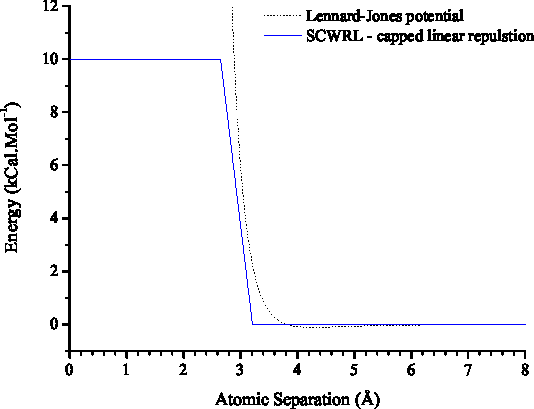
\includegraphics[width=0.7\textwidth]{./09-Arcus/scwrl/atom_interact.pdf}
\caption[The SCWRL capped linear-repulstion potential]{The \textsc{Scrwl} capped linear-repulsion potential: The example illustrated here is the comparison of the \textsc{Scrwl} form with that of a typical Lennard-Jones potential for two interacting alanine \sidechain\ methyl-groups, using parameters from the most recent \amber\ all-atom forcefield.}
\label{figure:arcus:scwrl:pair_energy}
\end{center}
\end{figure}

The \textsc{Scwrl} energy function is de-convoluted into both self and pairwise energy terms per-rotamer.
The probability-energy of a given rotamer is defined by the PDB-derived probability of the rotameric state ($E_\text{prob}$), in the context of the current \phipsi\ pair. The log is taken of the probability of each rotamer ($r_i$) divided by the probability of
most likely rotameric state.\begin{equation}
E_\text{prob}(r_i) = \log\frac{p(r_{i}\mid\phi,\psi)}{p(r_{i}=1\mid\phi,\psi)}
\end{equation}

The self steric interaction energy is that of the rotamer with any static atoms ($E_\text{self\_steric}$), typically the protein backbone, but in the case of \arcus\ also includes the heavy atoms in the \sidechains\ of the rigid body.
Importantly, the steric interactions ignore the two neighbouring residues (j=$i\pm1$), as it is assumed that the rotamer library itself will implicitly resolve these interactions.
Thus, $E_{sb}$ is defined as the summation of  $E_\text{contact}$  between each atom of the rotamer
($r_i$) and all static atoms in each \emph{active} residue $j$ such that $j<i-1$ and $j>i+1$.

\begin{equation}
E_\text{self\_steric}(r_i) = \sum_{j<i-1,\ j>i+1} E_{sb}(r_i,j)
\end{equation}

The two terms are summated after $E_\text{prob}$ is multiplied by a scaling factor $K$, resulting in a value for $E_\text{Self}(r_i),$ which describes each given rotamer in the context of the current protein environment.
$K$ was defined as 3.0 in the original publication and is, therefore, used in this work.

\begin{equation}
E_\text{Self}(r_i) = -KE_\text{prob}(r_i) + E_\text{self\_steric}(r_i) 
\end{equation}

The pairwise interaction between rotameric states is purely steric in nature. It is simply defined as the sum of $E_\text{contact}$ for each of the \emph{\sidechain} atoms in rotamer $r_i$ versus all of the \emph{\sidechain} atoms in rotamer $r_j$, where $i \ne j$. Thus, the complete energy of a complete set of rotamers within a given system is the sum of all self energies and the sum of all pairwise energies between all rotamers.

\begin{equation}
E_\text{System} = \sum_{i=1}^{n} E_\text{self}(r_i) +  \sum_{i=1}^{n-1}  \sum_{j>i}^{n} E_\text{pair}(r_i,r_{j}) 
\end{equation}

Proposed enhancements to \textsc{Scwrl} include the addition of further energetic terms to describe other important aspects in the determination of rotamer orientation, such as electrostatic and solvation effects. Importantly, neglect of these terms is most likely the reason that \textsc{Scwrl} performs significantly better on bulky residues where steric effects dominate rotamer orientation and significantly less well for residues like serine, where the orientation is dominated by electrostatic effects\cite{METHOD:SCWRL_2}.

\subsection{Dead-end Elimination via the Goldstein Criterion}

Dead-end elimination aims to remove all rotamers of residue $i$ for which it is certain that there is an alternative active rotamer, for the same residue, which has a lower interaction energy with the static atoms and all other active residues, \emph{regardless} of what rotamers are chosen for the active residues. Such a test requires surprisingly few comparisons and typically yields a reduction of approximately 80\% in active rotameric states.

The criterion states that each rotamer $s_i$ may be eliminated if the following holds true:

\begin{equation}
E_\text{self}(s_i)- E_\text{self}(r_i)+ \sum_{j=1,j\neq i}^{n}  \min \left\{ E_{\text{pair}}(s_i,r_j) -   E_{\text{pair}}(r_i,r_j) \right\}  >  0 
\end{equation}

In words; the sum of the minimum values of the difference in pairwise interaction energies
between the two rotamer states $s_i$ and $r_i$ is calculated. This is evaluated for every other residue $j$ by using any of its active rotameric states. By computing the minimised summation of these interactions and comparing it to the difference in self energies, it is known that the rotamer $s_i$ can can be eliminated if the resultant difference is positive. 

\subsection{Solving the Undirected Graph}
\label{section:arcus:graph_theory}

For this section, figure \ref{figure:arcus:graph_theory} is used to illustrate the use of graph theory within the \textsc{Scwrl} algorithm. The algorithm to compute biconnected components is described in the following sub-section. Following this, the use of such an algorithm as it pertains to \textsc{Scwrl} is defined.

\begin{figure}[hbtp]
\begin{center}
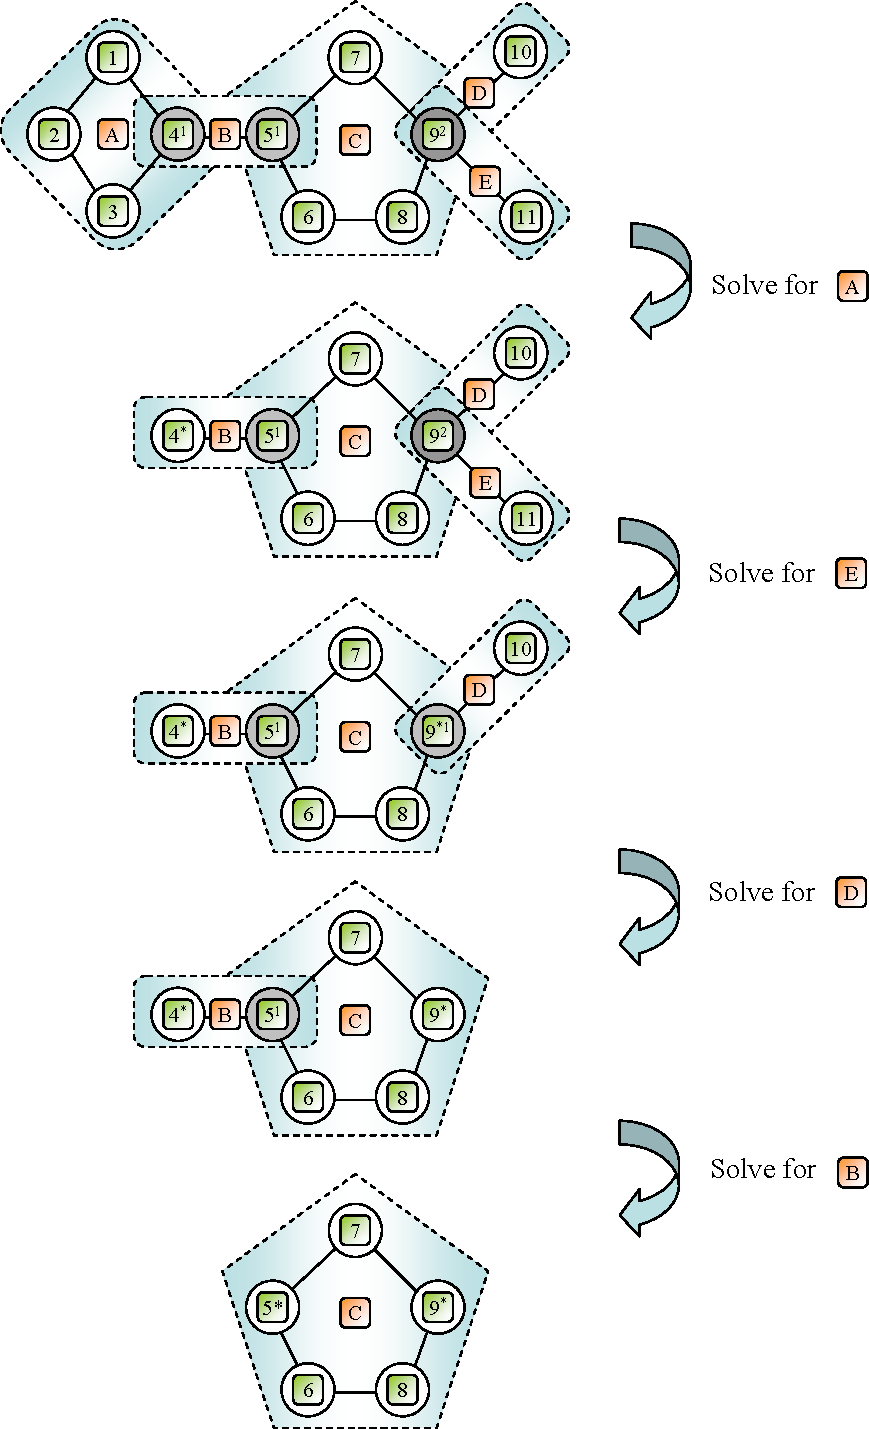
\includegraphics[width=0.78\textwidth]{./09-Arcus/scwrl/graph.pdf}
\caption[Solving a residue-interaction graph using \textsc{Scwrl}]{Solving a residue-interaction graph using \textsc{Scwrl}. \\
In the above diagram, each circle represents a vertex in the undirected graph, with edges represented as black lines. Each vertex represents a single amino acid and is labelled by the residue number in a green box. White, light grey and dark grey vertices represent zero, first and second order articulation points respectively.\ The articulation order is also shown by a superscript number. Blue dashed-line boxes represent individual biconnected components and are labelled using letters in orange boxes. Following the condensation of each satellite biconnected component onto each first order articulation point in turn, the articulation point is marked with an asterisk to signify that it is a super-residue.}
\label{figure:arcus:graph_theory}
\end{center}
\end{figure}

 
\subsubsection{Identifying Biconnected Components}

In order for \textsc{Scwrl} to break the system into manageable chunks, the biconnected components of the undirected graph and their articulation points must be identified. This is performed using a linear-time depth-first search algorithm developed by Tarjan\cite{METHOD:Tarjan1972}. The algorithm, which is shown as \CPP\-code in listing \ref{listing:arcus:tarjan}, functions via tree-traversal of the undirected graph:
\lstset{language=C++}
\begin{lstlisting}[float, caption={ \pd s implementation of Tarjan's algorithm for identifying biconnected components. The entry-point is calcBiConnections(). Prior to execution, m\_Vertices and m\_Edges must be filled with data and both m\_EdgeStack and m\_BiComponents cleared.}, label=listing:arcus:tarjan]
const int UNDEFINED = INT_MAX; // assign the undefined value as the largest number an int can hold
int m_CurrentDFN;
std::vector<Vertex> m_Vertices; // The member variable containing vertex definitions
std::vector<Edge> m_Edges; // The member variable containing edge definitions
std::vector<Edge> m_EdgeStack; // A temporary variable used by biConnect()
std::vector<BiconnectedComponent> m_BiComponents;

void UndirectedGraph::biConnect( int _v, int _u )
{
        Vertex& v = m_Vertices[_v]; // Obtain a reference to vertex-v
        v.dfn = ++m_CurrentDFN; // Assign a DFN to this vertex and increment the count
        v.lowpt = v.dfn; // Initially assign L(v) to the DFN, it may be reduced below...

        // For each vertex in the adjacency list of vertex-v...
        for( int i = 0; i < v.adjacency.size(); i++ )
        {
                int _w = v.adjacency[i];
                Vertex& w = m_Vertices[_w]; // Obtain vertex-w
                
                if( w.dfn == UNDEFINED ) // Vertex w is not yet assigned
                {
                        m_EdgeStack.push_back( Edge( _v, _w ) ); // add (v,w) to the edge stack

                        biConnect( _w, _v ); // A recursive call to this function
                        v.lowpt = min( v.lowpt, w.lowpt );

                        if( w.lowpt >= v.dfn )
                        {     
                                BiconnectedComponent bc; // A new component has been found!
                                
                                while( true ) // an infinite loop
                                {
                                        Edge& e = m_EdgeStack.back();
                                        if( m_Vertices[e.fromVertex].dfn >= w.dfn )
                                        {
                                                bc.edges.push_back( e );
                                                m_EdgeStack.pop_back();
                                        }
                                        else
                                        {
                                                break; // break out of the infinite loop
                                        }
                                }

                                // obtain the edge from the top of the edge stack 
                                // and add it to the biconnected component.
                                Edge& e = m_EdgeStack.back();
                                bc.edges.push_back( e );
                                m_EdgeStack.pop_back();

                                // Add this completed component to the main container
                                m_BiComponents.push_back( bc );
                        }

                }
                else if( w.dfn < v.dfn && _w != _u )
                {
                        m_EdgeStack.push_back( Edge( _v, _w ) );
                        v.lowpt = min( v.lowpt, w.dfn );
                }
        }               
}

void UndirectedGraph::calcBiConnections()
{
        // Flag all the vertices as un-traversed
        for( int i = 0; i < m_Vertices.size(); i++ )
        {
                m_Vertices[i].number = UNDEFINED; // Uninitialised
                m_Vertices[i].lowpt = UNDEFINED; // Uninitialised                       
        }
        
        calcAdjacency(); // Fill the adjacency list for every vertex from the current edge list

        // initialise member variables
        m_BiComponents.clear();
        m_CurrentDFN = 0;
        m_EdgeStack.clear();
        
        for( int i = 0; i < m_Vertices.size(); i++ )
        {
                if( m_Vertices[i].number == UNDEFINED ) // if still uninitialised
                        biConnect( i, 0 ); // then call biConnect() for vertex-i
        }
        calcArticulationOrders(); // Calculate articulation orders for each vertex
}
\end{lstlisting}

From an arbitrary starting vertex, using the adjacency list for each vertex, edges are traversed and the vertices numbered in the order they are visited -- termed the depth-first number (DFN). This process defines a tree, whereby each node in the tree may have multiple child nodes, but has only one parent. The tree is traversed to the greatest depth possible,  unexplored vertices are then considered, in the reverse order with respect to the order that their parents were traversed. An example of this can be given using figure \ref{figure:arcus:graph_theory}. Beginning arbitrarily from vertex 2 and depending on the exact ordering of each adjacency-list, the order of traversal may proceed: 2, 3, 4, 5, 7, 9, 10, 11, 8, 6, 1.
Note that during this search, the edges $5 \rightarrow6 $ and $1 \rightarrow2 $ are not traversed. In addition to the assignment of the DFN, each vertex is assigned a low-number, annotated $L(u)$, defined by equation \ref{eqn:arcus:tarjan}. 

\begin{equation}
L(u) =  \min \left\{ \begin{array}{ll}
 DFN(u) \\
\min (L(w) \mid w\ \text{is a child of}\ u)\\ \min(DFN(w)\mid (u,w)\ \text{is a back-edge}) \\
\end{array}
\right.
\label{eqn:arcus:tarjan}
\end{equation}


$L(u)$ is essentially the lowest DFN that can be achieved by the traversal from $u$ on a path that uses only the descendants of $u$ and at most one back-edge. It follows that each node $u$, which has a child $w$ with $DFN(u) < L(w)$, is either the root node or an articulation point. During traversal, each edge is added to a stack. When an articulation point is encountered, the edges relating to the current biconnected component will reside at the top of this stack. A new biconnected component is created, the edges are popped from stack and their vertices added to the new component. Thus, after the iterative search is complete, all biconnected components will have been defined along with all articulation points.
The order of each articulation point can then be simply calculated from the number of components in which it is a member vertex.

\subsubsection{Condensing the Graph}

The main purpose of figure \ref{figure:arcus:graph_theory} is to illustrate how, following identification of biconnected components, the graph can be condensed, one component at a time, until only a single biconnected component remains. The algorithm continually cycles through the list of biconnected components where,  each time it finds an unused component with only one articulation point, it performs a branch-and-bound search (section \ref{section:arcus:scrwl:branch_bound}) and then marks the component as used. The search is performed over all possible rotameric states for all residues in that biconnected component, with reference to the articulation point. This eventually yields the optimal combination of rotamers for each possible rotameric state of the articulation residue. Following this, the articulation point becomes a vertex with an articulation order of zero, but is now a super-residue, where each of its rotameric states now includes the optimal set of rotameric states for all child residues. The self-energy for this super-residue is now defined as the summation of its own self-energy, the self-energies of all its children and all pairwise interactions within the biconnected component. 

When only one biconnected component remains, the branch-and-bound search is repeated one last time. Following this the best rotamer for the final condensed vertex is selected, whereby within this single super-vertex, the globally optimal arrangement of all child residues is contained, which by definition includes all the residues within the entire connected component.


\subsection{Branch and Bound}
\label{section:arcus:scrwl:branch_bound}

The final procedure to discuss, which completes the definition of the \textsc{Scwrl} algorithm, is the branch-and-bound search method. This solves the optimal arrangement of rotamers for each biconnected component with respect to its primary residue. The primary residue is defined as the articulation point for all but the final component, when the residue with the smallest number of active rotameric states is chosen. 

A branching pattern is defined by the number of residues in the biconnected component and the number of rotamers each one has. Figure \ref{figure:arcus:scwrl:branch_bound} shows the branches for a four residue biconnected component.
To increase the rate at which the branch-and-bound algorithm is able to back-track and eliminate branches, the residues are considered in order from the lowest to highest total active rotamers. The rotamers are then considered in order from the lowest to highest self-energies. 
\begin{figure}[hbtp]
\begin{center}
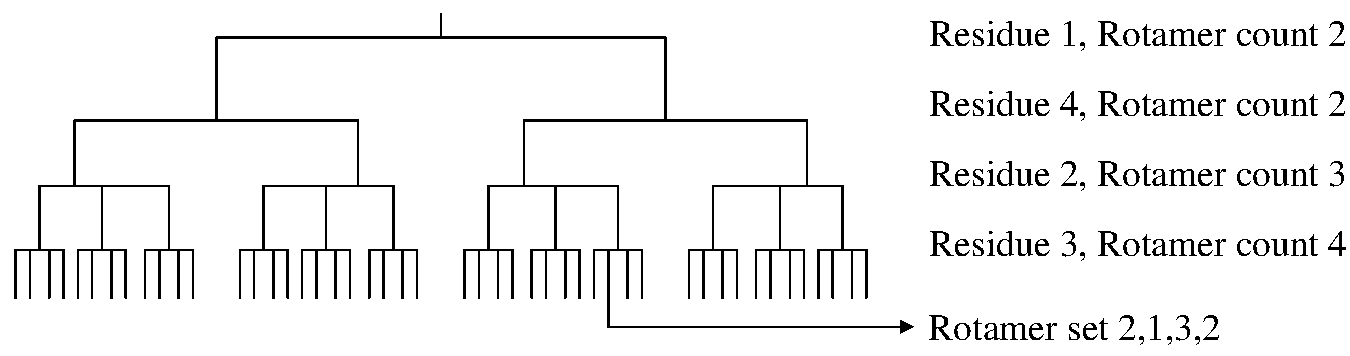
\includegraphics[width=0.85\textwidth]{./09-Arcus/scwrl/branch-and-bound.pdf}
\caption{A tree representing the rotamer interactions for an interacting set of residues.}
\label{figure:arcus:scwrl:branch_bound}
\end{center}
\end{figure}

The tree is recursively enumerated and at each level, the summed energy is checked by a bounding function to see if the minimum energy for the branches below it is larger than the best energy found so far. If it is, then no further nodes of the current branch are traversed. The previous sorting operations ensure that this occurs as frequently as possible. The bounding function is defined by equation \ref{eqn:arcus:scwrl:branch_bound}.
 
\begin{equation}
E_\text{bound}(i) = \sum_{j>i} \left\{ \min_{rj} E_\text{self}(r_j) \right\} +  \sum_{j>i} \sum_{k<j} \left\{ \min_{rj,rk} E_\text{pair}(r_j,r_{k}) \right\} \label{eqn:arcus:scwrl:branch_bound}
\end{equation}


\section{Additional Enhancements}

The following two sub-sections detail additional enhancements which were implemented for \arcus.

\subsection{An Updated Re-join Force}
\label{section:arcus:rejoinforce}

The loop re-join force in \arcus\ was completely revamped from its original incarnation in \prearcus. It now exhibits three main differences, but still utilises the same mathematical form and restraint implementation. As stated in section \ref{section:arcus:dualbranch}, the \mainchain\ break is now in the centre of the loop, as opposed to the C-terminus, but still crosses the \Omg-torsion.
In light of this, the first change is that, as opposed to the use of \emph{absolute} Cartesian restraints, the new version must use \emph{relative} Cartesian restraints -- essentially that atom-$a$ must be approximately $d$\AA\ from atom-$b$, as opposed to atom-$a$ must be within $d$\AA\ of Cartesian coordinate \textless$x$,$y$,$z$\textgreater. In \prearcus\ these absolute coordinates were set from the \xray\ structure.
In \arcus\ such information is obviously no longer available, as the Cartesian coordinates for the join-location are unknown.

Secondly, the atoms which are restrained are now different. \prearcus\ restrained the O and C-atoms of the C-terminal residue to the locations found in the \xray\ structure. In order to ensure that a planar peptide-group is re-created at the break, more
restraints are required. Essentially, a distance matrix was formed for the atoms C$_\alpha^{(n-1)}$, C$^{(n-1)}$, O$^{(n-1)}$, N, H, and C$_\alpha$, where the restrained distances were obtained from averaged high-quality \xray\ structures.
This matrix is sufficient for the formation of a trans-peptide bond. The cis-peptide bond is ignored, as its is not represented in the optimal 8-10-5 \angleset\ in any case, for reasons discussed previously in section \ref{section:reduced_rep:optimised_angleset}. In the special case of Proline, there is no H atom and so the restraints involving this atom are ignored. For this reason, both the  cis and trans-peptide conformations can form during torsional minimisation.

Finally and most significantly, not only is the break itself restrained, but also the \ca\ positions of the loop \mainchain. The reason behind this decision was that, in \prearcus, it was sometimes found that either strong steric interactions or the re-join force would cause large Cartesian shifts in loop conformation.\ The atomic forces, however,  can often be satisfied without such excessive displacement from the starting conformation, which \emph{critically} has already passed all stage 1 conformational filters. In order to combat this undesirable trait, the \ca-atom restraints are used to disfavour the loop traveling too far from its starting conformation. With these in place, more subtle torsional changes can then occur to allow the break to be sealed whilst also calming any moderate steric interactions.

\subsection{Rationale for Clustering}
\label{section:arcus:cluster}

Crystal structures are, by definition, static. However, real proteins are known to be highly dynamic structures in aqueous solution. The native state is thought to be an ensemble of highly similar structures with low free energy. To capture the essence of this ensemble in a single snapshot is a difficult task. Many modelling methods rely solely on the internal energy of a given structure -- a single energy minimum. Real energy minima are a function not only of the internal energy of a given structure, but also the conformational entropy of the ensemble. Rather than describing single minima, an ensemble  instead describes \emph{valleys} on the potential energy surface. That is to say the more low energy structures found within a given ensemble, the more entropically favourable it is, the converse is also true.



A crude, but highly effective form of clustering is invoked following the production of joined conformations at the end of stage 2. For any clustering algorithm, for efficiency, it is critical that the number of pair-wise comparisons be minimised. In this case, clustering was performed on the basis of \mainchain\ heavy-atom RMSD. The list of conformations was first sorted by energy, lowest first. This energy included the torsional, steric terms and any Cartesian restraint terms. Next, starting at the beginning of the sorted list, the first structure was marked as the primary. The current primary structure is deemed a cluster centre. Proceeding down the list, each conformation under 0.25\AA\ RMSD to the primary structure was included in the same cluster and flagged as taken. Next, the algorithm returns to the beginning of the list and proceeds along it until it encounters a conformation which is not flagged as taken. This structure is then marked as primary and the procedure continues until all structures are marked as taken. The list of cluster representatives is then simply all the conformations which were marked as primary at any point.
Due to the initial sorting of the list, the representatives will be the lowest steric-energy structures in their cluster. These representatives are then sent to stage 3 for refinement. By using the energy as the determinant for cluster centres, the number of pairwise \crms\ comparisons is vastly reduced, whilst ensuring that each cluster center is suitably different prior to further refinement.





\section{ Full Implementation Details}
\label{section:arcus:exactImplementation}

The following sub-sections define the control logic used within \arcus\ and how each individual component, described by the preceding sections, is integrated within the protocol.

\subsection{Stage 1A -- Branch Generation}

 In what is termed stage 1A, the N and C-terminal conformer branches are initially generated separately, each assessed under its own set of conformational filters. The Cartesian coordinates of any viable conformations are stored in a memory buffer. The exact array of filters which are currently used are as follows: 

\begin{enumerate} \isep
\item 
A \mainchain\ self-clash filter with an overlap factor of 0.65. This ensures that the branch does not clash with itself.\item
The branch-distance filter, exactly as described in section \ref{section:arcus:branchDistFilter}.\item
The over-extension filter, exactly as described in section \ref{section:arcus:overExtFilter}.\item
The clash-grid filter, exactly as described in section \ref{section:arcus:clashGridFilter}. This was initialised with a atom inclusion cutoff of 3.5\AA\ for each grid point and a steric overlap-factor of 0.65.
\end{enumerate}


\subsection{Stage 1B -- Branch Pairing}

Following the generation of fifty valid conformations for both the N and C-terminal branches in stage 1A, stage 1B assesses each possible pairing of N and C-terminal branches for the ability to join, defined by an N--C distance of \textless1.5\AA\ across the chain-break.
The pair is then assessed for steric conflict over all heavy \mainchain\ atoms. If this filter passes, the rotamer packing algorithm, as described in section \ref{section:arcus:impRotPack}, is then re-invoked on the entire loop. This ensures that there is at least one \sidechain\ conformation for each residue which fits within the available volume; given the current \mainchain\ conformation.
Two further clash filters are then called in turn. The first considers all heavy atoms in either branch, the second checks for steric interactions between the loop and the static atoms using a clash-grid. Conformations which pass these filters are stored for refinement in stage 2. 

Stage 1A and 1B are repeated, testing all conformers which have not been compared from both the N and C-terminal buffers at each iteration, until $x$  complete conformers have been added to the buffer. These conformations all have the potential to be re-joined during stage 2. The optimal value for $x$ is discussed later in section \ref{section:arcus:nummod}.



\subsection{Stage 2A -- Torsional Re-join}

Just as in \prearcus, stage 2A essentially remains  a sterically-guided torsional energy minimisation of any conformation which has the potential to be re-joined. There are, however, a number of important differences. Firstly, the starting conformation is now refined to a much greater extent -- the job of the minimisation is now focused on performing the re-join itself as opposed to calming steric interactions. Secondly, the re-join force is now as described in section \ref{section:arcus:rejoinforce}, including \ca-atom restraints over the entire loop. Finally, stage 2 now contains three post-filters which are designed to test whether the loop has been joined and if, in the process of doing so, has strayed too far from acceptable values for selected conformational properties.

These filters begin by firstly performing an assessment of whether the rejoin has been successful. This is done by analysing the distance matrix of the atom positions in the broken $\Omega$-bond. The values are compared to averaged values taken from \xray-structures. The torsion of the bond is also assessed, whereby a maximal deviation of 25\degree\ is tolerated, derived from figure \ref{fig:reducedrep:omg}.
Next, an \angleset\ filter is imposed which checks that all \phipsi\ torsions are within a 50.0\degree\ radius of any parametised angle, for the same residue-type, within the current \angleset. This is especially important for the residues at either side of the join, as their \phipsi\ angles are defined during the torsional minimisation. Finally, the over-extension filter used by \mbox{stage 1} is re-invoked to test for occasional gross displacement during the torsional minimisation.

\subsection{Stage 2B -- Clustering}

Stage 2 concludes with the clustering process outlined in section \ref{section:arcus:cluster}, termed stage 2B. Using a tight similarity cut-off of 0.25\AA, very similar structures are removed, whereby only the cluster representatives are sent to stage 3 for refinement.

\subsection{Stage 3 -- Detailed Refinement}
\label{section:arcus:stage3}

In \arcus, stage-3 has been replaced with a plug-and-play refinement system. The default refinement plug-in is essentially that used previously in \prearcus\ --   remaining a randomised sampling around a sterically-valid  joined conformer, where all structural perturbations have been retained in the same format except for the randomised rotamer application.
The rotamer perturbation is replaced with a low probability that \textsc{Scwrl} will be invoked on the loop conformation. The other main difference is that the standard metropolis MC protocol within \pd\ is used to drive the perturbation process with standard acceptance criteria. Additional refiners have also been defined: 

The first additional refiner is simply a call to \textsc{Scwrl} followed by Cartesian conjugate energy minimisation. This time, a more fine-grained version the rotamer library is used. This refiner has been used in this chapter to give performance statistics for the stage 2 conformers when selected using the \ambergbsa\ \forcefield, without the addition of the MC sampling routine. This, therefore, shows the raw performance improvements obtained by the new components implemented for stages 1 and 2.

The second refiner is important for the computational parallelisation of \arcus\ -- allowing stages 1 and 2 to be segregated from the stage 3 refinement process and the refinement to be split over multiple computers. In this case the refiner actually performs no refinement, but instead saves the structural data to a trajectory file for later use. The joined stage 2 conformations can then be recalled and potentially later assessed under multiple different refiners as desired. In order to ``replay'' the trajectory, a second protocol \textit{ArcusReplay} is given the trajectory and one of the refiners. It then loads each stage 2B joined conformation in turn and invokes the chosen refiner upon it.
As usual, the single lowest energy conformation visited during the refinement is kept as the final model.

\section{Results and Discussion}

In this section, the final predictive performance of \arcus\ 1.0 is presented. Some of the calibrations described below used a reduced set of either 100 or 250 randomly selected \mer{8} loops, which were selected from \thothloopdb. It is assumed that the data obtained for these reduced sets are equally representative of the entire population of loop structures.
\subsection{The Optimal Number of Stage 1 Models}
\label{section:arcus:nummod}

Figure \ref{fig:arcus:optnummodel} shows the data that were used to determine the optimal number of models to generate during stage 1. This optimum is defined as the lowest count which gives good coverage of conformational space, defined via an analysis of the spread of RMSD values within the generated ensemble.
For 100 test loops, $x$ models were generated and the \mainchain\ and heavy-atom RMSD measured for all structures. The average, maximum and minimum of these RMSD\ values was then taken for each loop candidate in turn. The average of these quantities over \emph{all} loop candidates was then measured and plotted against $x$ in figure \ref{fig:arcus:optnummodel}, where $x$ was assigned values between 1 and 2000.

In the figure, it can be seen that the maximum and minimum plateau. The point at which the RMSD values approximately reach a plateau is assumed to be the point at which gross conformational space has been covered within the ensemble of model structures. From this criterion, it was decided that a total of 1,000 models per target structure should be generated to allow good coverage of conformational space. Of course, further structures would give slightly better coverage, but greatly increase the computing resources required.
\begin{figure}[hbtp]
\begin{center}
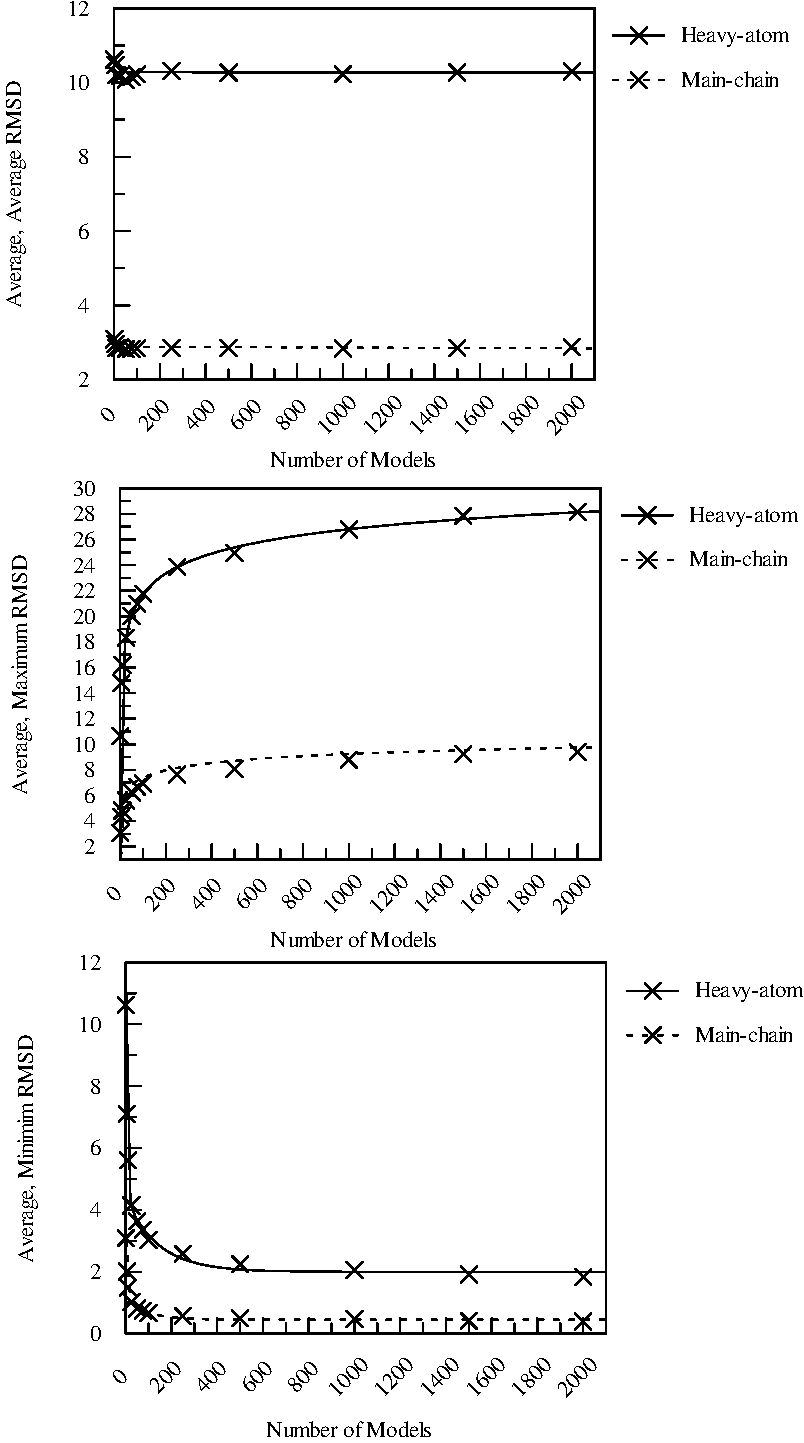
\includegraphics[width=0.76\textwidth]{./09-Arcus/num_mod/num_mod.pdf}
\caption[An analysis of the number of models required from stage 1]{An analysis of the number of models required from stage 1. The random selection of 100 \mer{8} \thothloopdb\ loops was used. For each target loop, $x$ models were requested which would pass all stage 1 filters; a wide range of $x$ values were used. Within these models, the average, minimum and maximum was calculated for both the Cartesian \mainchain -only and heavy-atom \crms\ measurements. The resultant six curves are shown in the graphs above. (Fitting was performed using arbitrary functions.)}
\label{fig:arcus:optnummodel}
\end{center}
\end{figure}

\subsection{Quality Improvement Following Filter Enhancement}

Next, the predictive performance increase resulting from the use of the new types of conformational filter are presented in table \ref{table:arcus:filterPerformance}. A significant improvement in the average values is seen for both filters individually and
further improvement is
seen when both are used together. This suggests that they are successfully filtering against different aspects of non-native conformation.\begin{table}[hbtp]
\begin{center}
\begin{tabular}{+l^c^c^c^c^c^c}
\toprule
\rowstyle{\bfseries}
\multirow{2}{*}{   
Filter
}
  & \multicolumn{3}{c}{\textbf{Main-chain (\AA)}} & \multicolumn{3}{c}{\textbf{Heavy-atom (\AA)}} \\
\rowstyle{\bfseries}
                &  Min.  &  Ave.  &  Max.  &  Min.  &  Ave.  &  Max. \\
\midrule
Standard  &  0.49  &  \textbf{3.21}  &  8.93  &  2.34  &  \textbf{11.58}  &  26.58 \\
 + Branch-distance Filter   &  0.43  &  \textbf{3.12}  &  8.40  &  2.20  &  \textbf{11.21}  &  26.01 \\
+ Over-extension Filter  &  0.52  &  \textbf{3.00}  &  8.62  &  2.42  &  \textbf{10.72}  &  25.72 \\
Both  &  0.50  &  \textbf{2.84}  &  8.07  &  2.25  &  \textbf{10.27}  &  24.97 \\
\bottomrule
\end{tabular}
\caption[RMSD changes under the new filter configuration.]{\crms\ changes under the new filter configuration. For the 100 \mer{8} loops, randomly selected from \thothloopdb, 500  \emph{valid} conformers were generated. Each valid conformer passed the stage 1 filters listed in column 1 of this table. For the selected conformers, for each of the 100 test loops, the average \crms\ of the valid ensemble was measured (\mainchain\ and heavy-atom \crms\ presented separately). The minimum, average and maximum over the range of 100 averages was then taken; this is presented above. In terms of filters, ``standard'' refers to the filters used in \prearcus, but now with the enhancements outlined in section \ref{section:arcus:filterdev}. The over-extension and branch-distance filters are considered both independently and then in collaboration. The measured averages, being most representative of the distribution, are shown in bold. When both filters are used combination, all average \crms\ values improve, illustrating a synergistic importance in the build process.}
\label{table:arcus:filterPerformance}
\end{center}
\end{table}


\subsection{Predictive Performance}

In chapter \ref{chapter:methods}, it was shown that whilst \prearcus\ performed reasonably well on shorter \mer{6} loops, but its predictive performance decayed more rapidly with increasing loop lengths when compared to other methods. It was also noted that the torsional quality of the generated models was poor.

For this chapter, \arcus\ was applied to on 250 randomly selected \mer{8} loops using the Cartesian minimisation refiner described in section \ref{section:arcus:stage3}. 
For consistency, the measures of structural similarity to the native state are exactly the same as those described in chapter \ref{chapter:methods}. Figure \ref{figure:arcus:compPrearcusArcus} shows a significant increase in predictive performance for \mer{8} loops; gained from the enhancements now implemented in \arcus. It can now be seen that on average much lower Cartesian \crms\ structures are generated. It is also clear that native-like \mainchain\ torsions are now generated to a far greater extent. 

\modloop\ was the most effective method assessed during the critical loop modelling method assessment presented in chapter \ref{chapter:methods}. Thus, in figure \ref{figure:arcus:compModloopArcus}, the new results for \arcus\ is compared to \modloop\ with the \textsc{Dope} forcefield.
 Although each method uses an entirely different protocol, the results are now very similar.
\modloop\ produces a slightly greater fraction of very low \crms\ structures, however the fraction of predictions which may be deemed essentially correct is approximately the same. This shows that the predictive performance of \arcus\ is now comparable to the best methods currently available.

\begin{figure}[p]
\begin{center}
\subfigure[\prearcus\ Main-chain \crms]{
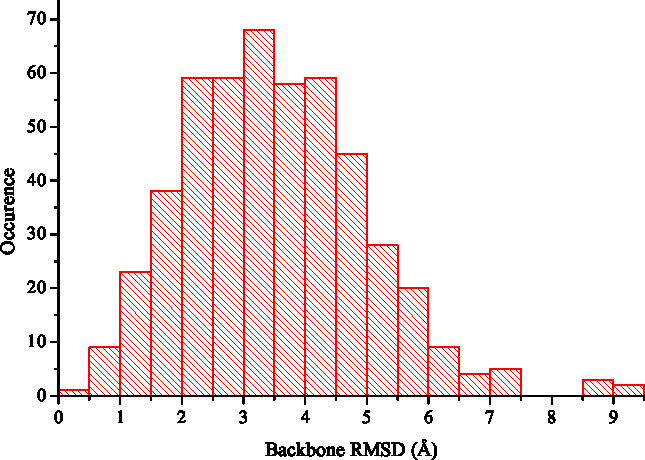
\includegraphics[width=0.45\textwidth]{AppendixA/prearcus/amber-ua/bb_8_PreArcus.pdf}}
\subfigure[\arcus\ Main-chain \crms]{
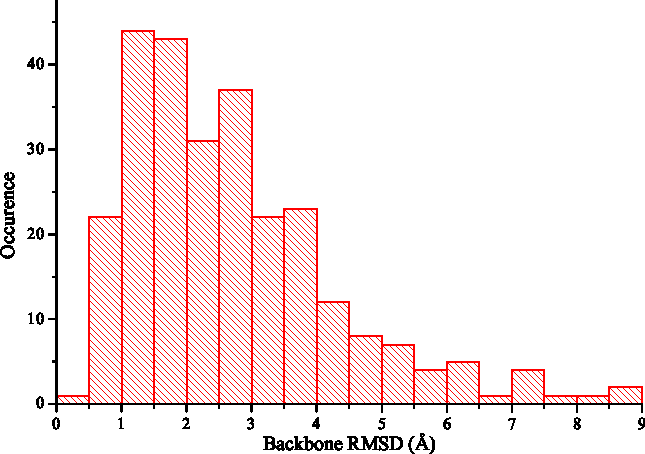
\includegraphics[width=0.45\textwidth]{09-Arcus/result_noMC/bb_8_Arcus.pdf}}
\subfigure[\prearcus\ Heavy-atom \crms]{
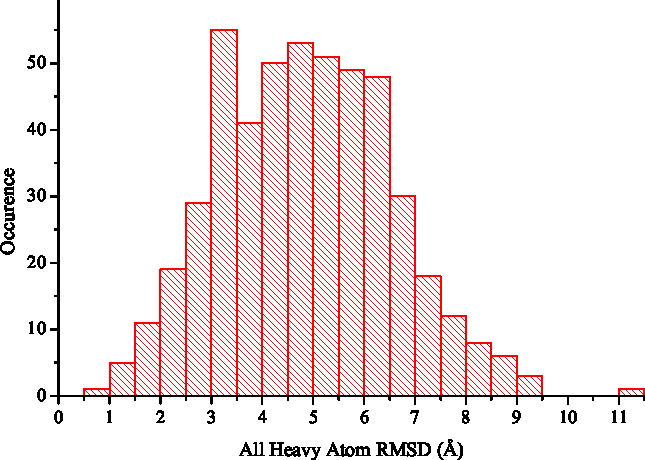
\includegraphics[width=0.45\textwidth]{AppendixA/prearcus/amber-ua/aa_8_PreArcus.pdf}}
\subfigure[\arcus\ Heavy-atom \crms]{
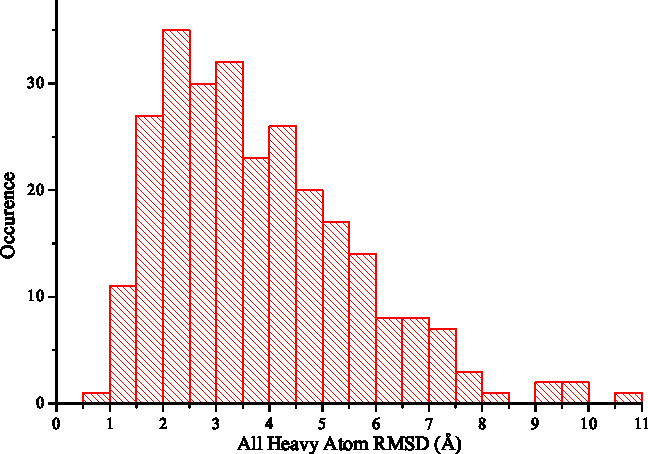
\includegraphics[width=0.45\textwidth]{09-Arcus/result_noMC/aa_8_Arcus.pdf}}
\subfigure[\prearcus\ Main-chain \arms]{
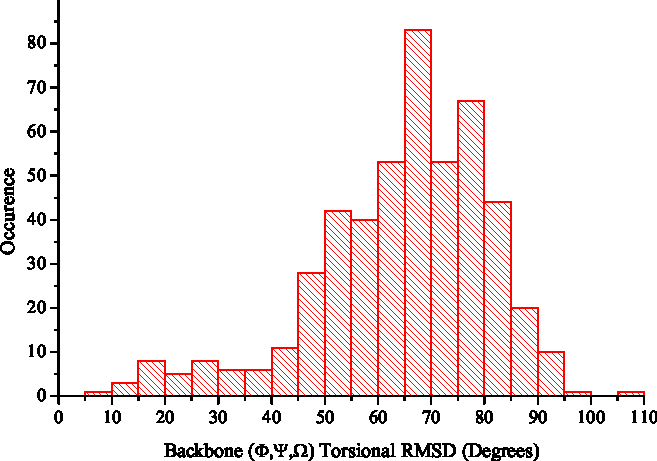
\includegraphics[width=0.45\textwidth]{AppendixA/prearcus/amber-ua/bba_8_PreArcus.pdf}}
\subfigure[\arcus\ Main-chain \arms]{
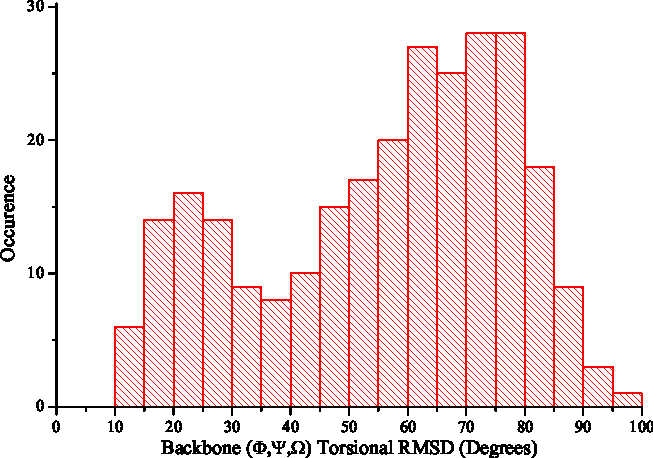
\includegraphics[width=0.45\textwidth]{09-Arcus/result_noMC/bba_8_Arcus.pdf}}
\end{center}
\caption[Comparing the predictive performance of \prearcus\ and \arcus\ on \mer{8} loops.]{Comparing the predictive performance of \prearcus\ and \arcus\ on \mer{8} loops. A significant improvement can be seen, especially for the torsional measure, which now exhibits a far stronger native-like signal.}
\label{figure:arcus:compPrearcusArcus}
\end{figure}

\begin{figure}[p]
\begin{center}
\subfigure[\modloop\ Main-chain \crms]{
\includegraphics[width=0.45\textwidth]{AppendixA/modloop/dope/bb_8_modloop.pdf}}
\subfigure[\arcus\ Main-chain \crms]{
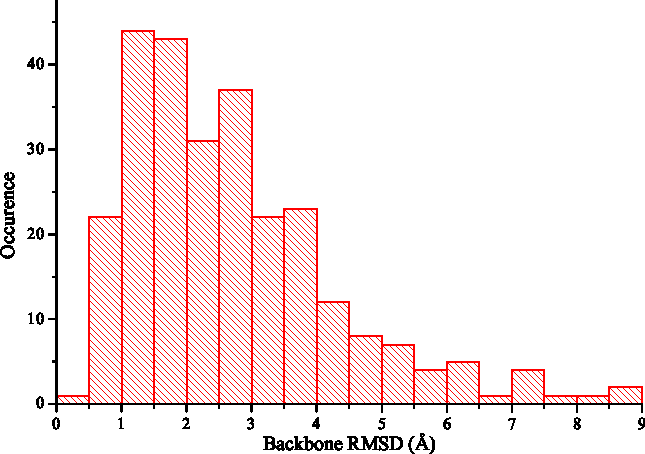
\includegraphics[width=0.45\textwidth]{09-Arcus/result_noMC/bb_8_Arcus.pdf}}
\subfigure[\modloop\ Heavy-atom \crms]{
\includegraphics[width=0.45\textwidth]{AppendixA/modloop/dope/aa_8_modloop.pdf}}
\subfigure[\arcus\ Heavy-atom \crms]{
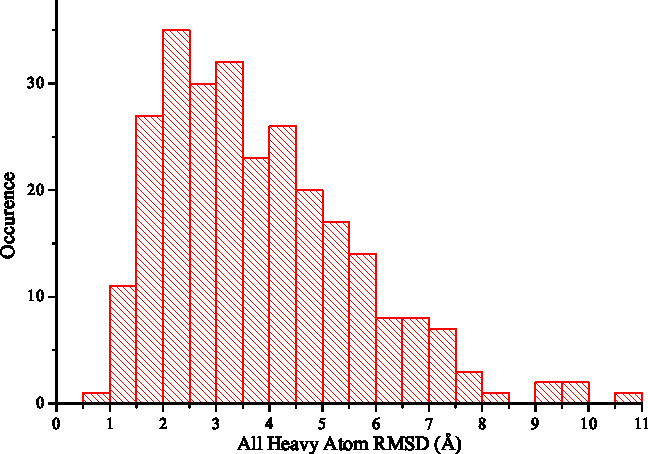
\includegraphics[width=0.45\textwidth]{09-Arcus/result_noMC/aa_8_Arcus.pdf}}
\subfigure[\modloop\ Main-chain \arms]{
\includegraphics[width=0.45\textwidth]{AppendixA/modloop/dope/bba_8_modloop.pdf}}
\subfigure[\arcus\ Main-chain \arms]{
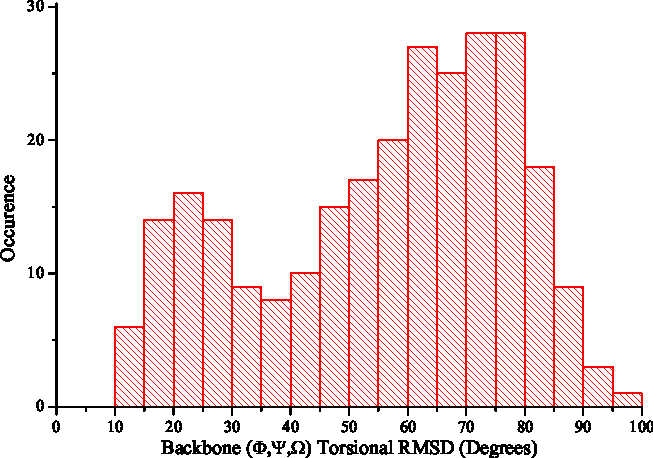
\includegraphics[width=0.45\textwidth]{09-Arcus/result_noMC/bba_8_Arcus.pdf}}
\end{center}
\caption[Comparing the predictive performance of \modloop\ and \arcus\ on \mer{8} loops.]{Comparing the predictive performance of \modloop\ with the \textsc{Dope} \forcefield\ and \arcus\ on \mer{8} loops. \modloop\ was the best performing method assessed for chapter \ref{chapter:methods}.}
\label{figure:arcus:compModloopArcus}
\end{figure}


\section{Final Remarks}

Three main performance enhancing improvements were made during the transition from \prearcus\ to \arcus. The first was that structural filters were tightened and torsional exploration was allowed during stage 1. Critically, this facilitated the generation of native-like conformations which simultaneously satisfy geometric and steric constraints in the context of the protein body.
The second was a computationally efficient rotamer assignment algorithm. Use of this algorithm ensured that there was sufficient space to place all \sidechains\ and that the optimal arrangement was produced. Finally, additional conformational filters were developed, ensuring that non-native-like structures were discarded as early as possible in the search process.


Following these improvements to the conformational search process, the predictive performance of \arcus\ is now comparable to that of \modloop. It is likely that the limiting factor is now the quality of the \forcefield\ used for assessment, as opposed to the conformational search itself.



